\documentclass{article}
\usepackage[a4paper, total={6.5in, 10.5in}]{geometry}
\usepackage{graphicx}
\usepackage{multirow}

\author{Katarzyna Macioszek, Ada Majchrzak}
\title{Data Mining project - part II}

\begin{document}
	\maketitle
	
	\section{Introduction}
	In the second part of the project we will use cluster analysis in connection with dimension reduction methods on \textit{Spambase} dataset. Our goal is to asses clustering algorithms performance in differentiation between \textit{spam} and \textit{nonspam} types. For that we shall use \textit{k-means}, PAM and AGNES clustering algorithms. We will also evaluate the quality of obtained results by checking separation measures of clusters built using original data and data after dimensionality reduction done with PCA algorithm. Additionally, we will also compare the results of classification performed on the former part of the project versus how the same methods will perform after applying dimensionality reduction.
	
	\section{Data preparation}
	To be consistent with analysis done in previous part of the project we again exclude columns that exhibit high correlation with each other. These eliminated features are \textit{num415} and \textit{num857}. Furthermore, we also use the same data transformations: z-score standardization and $\log(x+0.1)$ transformation to make the explanatory variables have comparable values, as it is crucial for clustering and dimensionality reduction algorithms.
	
	\section{PCA}
	To be able to visualize the multidimensional data easily and reduce the noise in our data before applying the clustering algorithms, we start with performing the principal component analysis (PCA). As mentioned before, we use two data transformations, however to display an interesting behavior of the method, let us first present the outputs for non-transformed data. To visualize PCA results we will use scree plot (Figure \ref{fig::screeplot}) and contributions of variables to the first two principal components (Figure \ref{fig::varplot}).
	
	\begin{figure}[h]
		\centering
		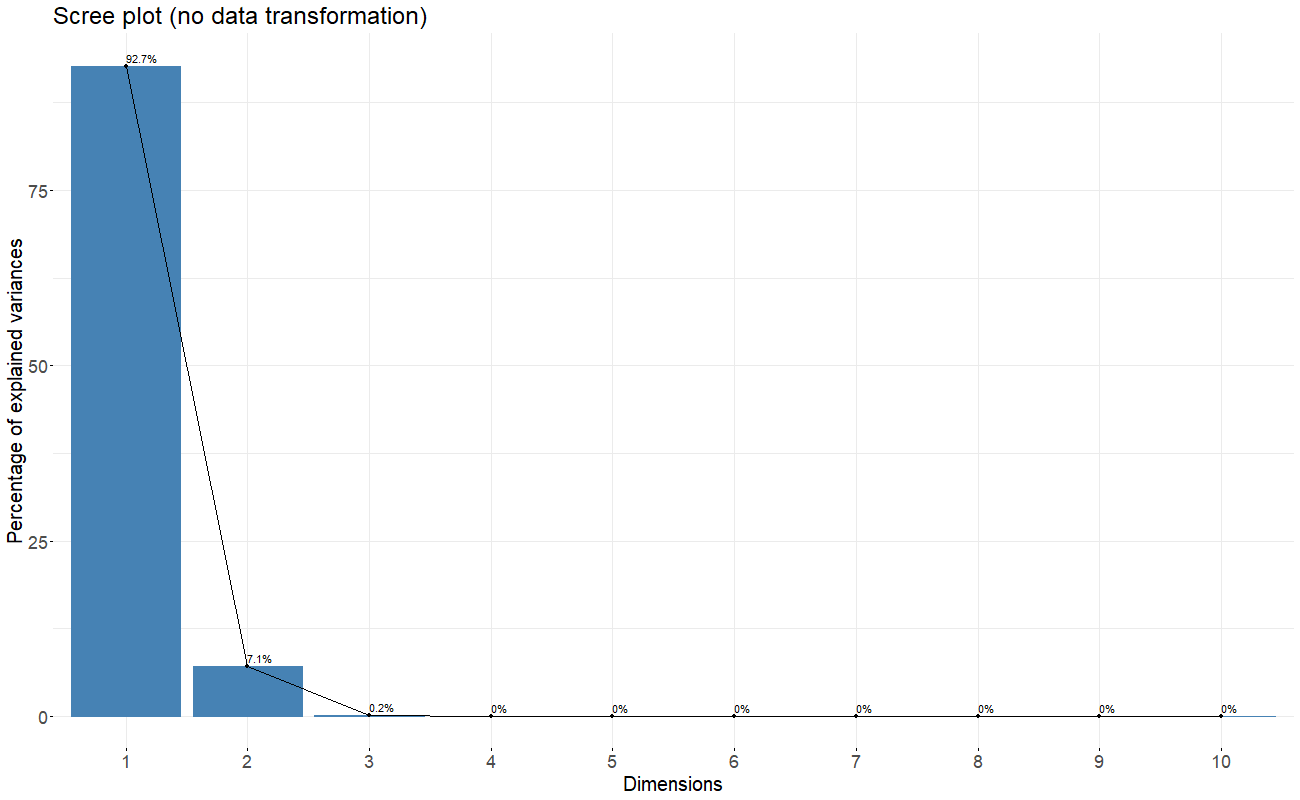
\includegraphics[width=0.9\textwidth]{proj2_plots/screeplot1.png}
		\caption{PCA results for original data (scree plot)}
		\label{fig::screeplot}
	\end{figure}
	
	\begin{figure}[h]
		\centering
		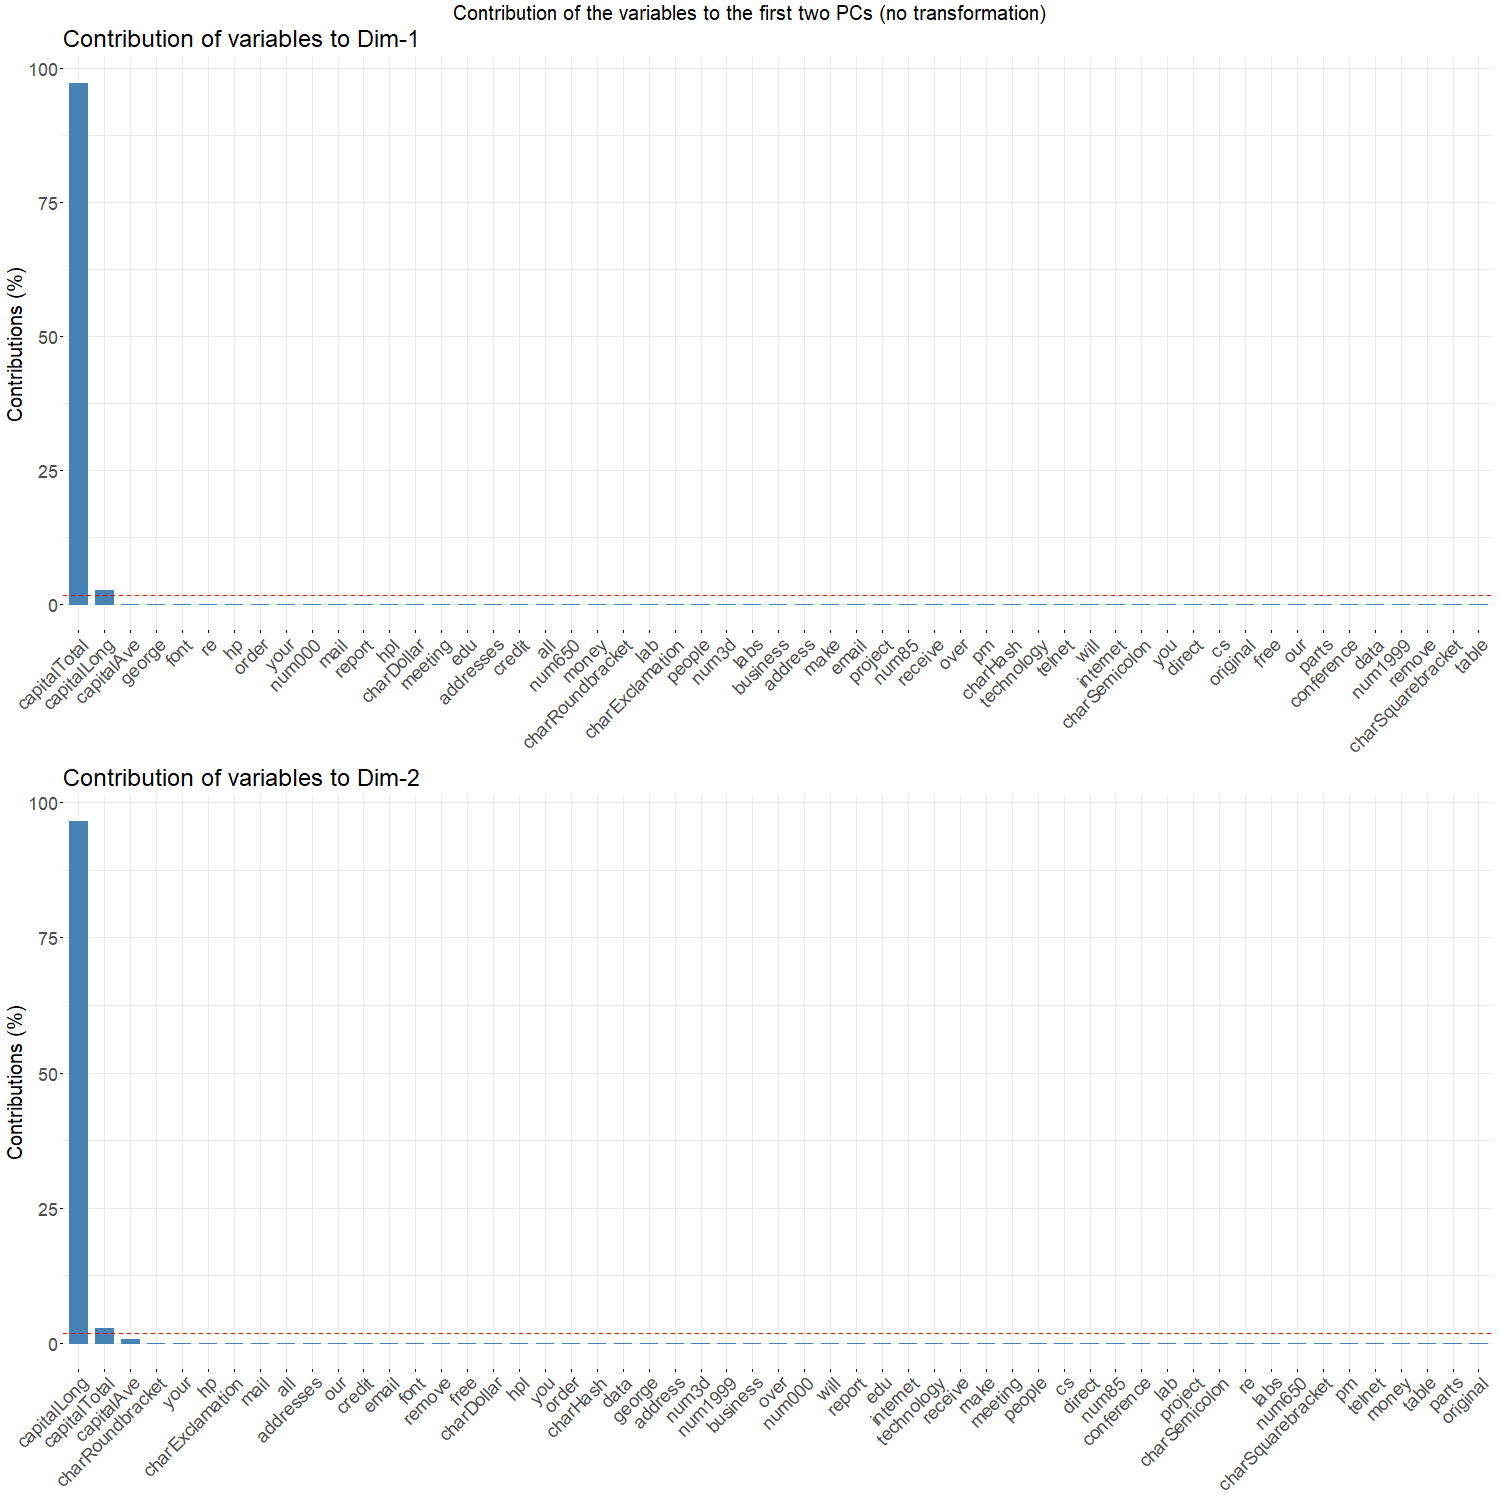
\includegraphics[width=0.9\textwidth]{proj2_plots/varplot1.png}
		\caption{PCA results for original data (variable contribution plot)}
		\label{fig::varplot}
	\end{figure}
	
 	
	As we expected, the algorithm gives poor results as only variables with highest spread are taken into consideration. In our data set most of the variables are frequencies with values in interval $[0, 100]$ and relatively low variance, and only capital letters characteristics have wider range of values. That causes the observed  behavior of PCA method, which results with only $2$ principal components, so in the following analyses we will use only transformed data.
	
	Let us now check the principal components for data after z-score standardization. The screeplot is displayed on Figure \ref{fig::varplot_zscore},
	while the variable contribution plot can be found on Figure \ref{fig::varplot_zscore}.
	As we anticipated, in this case we get more principal components created and also increased number of features is taken into account.

	\begin{figure}[h]
		\centering
		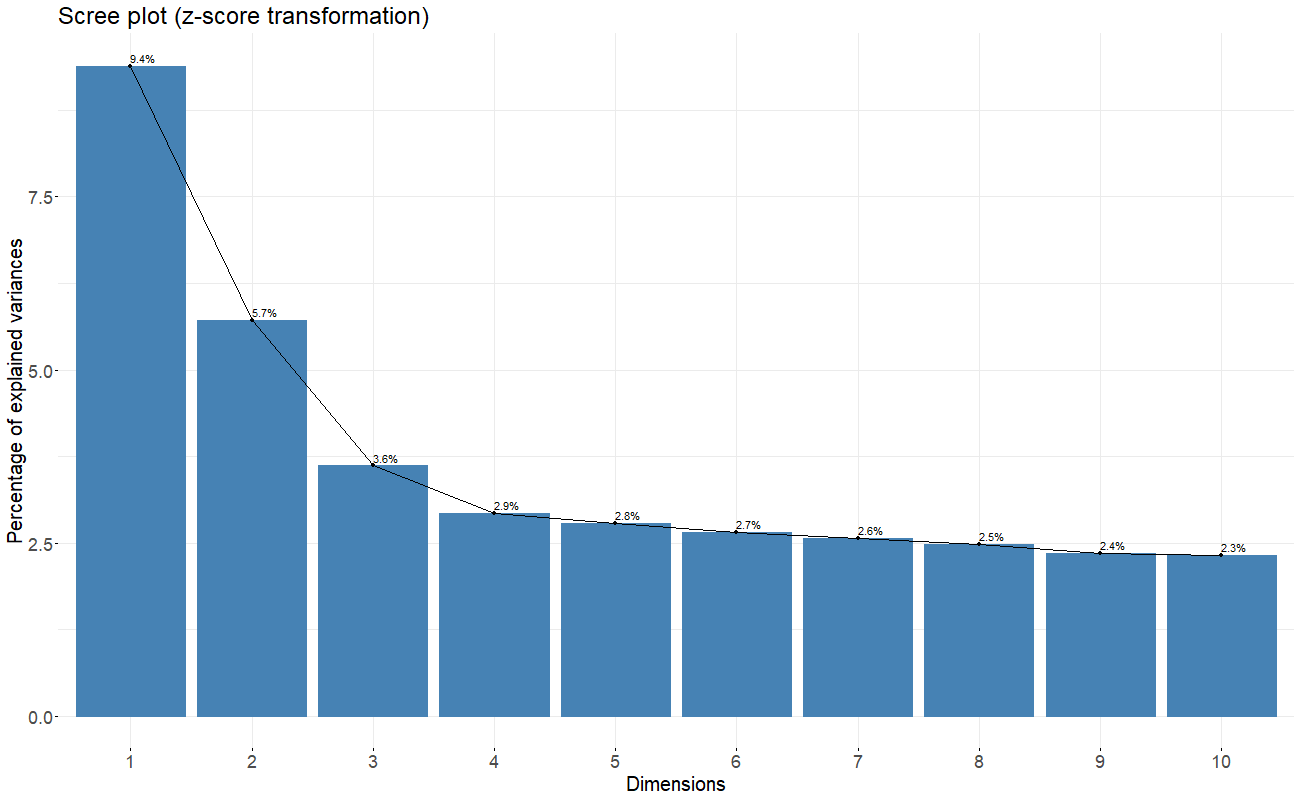
\includegraphics[width=0.9\textwidth]{proj2_plots/screeplot2.png}
		\caption{PCA results for standardized data (scree plot)}
		\label{fig::screeplot_zscore}
	\end{figure}
	
	\begin{figure}[h]
		\centering
		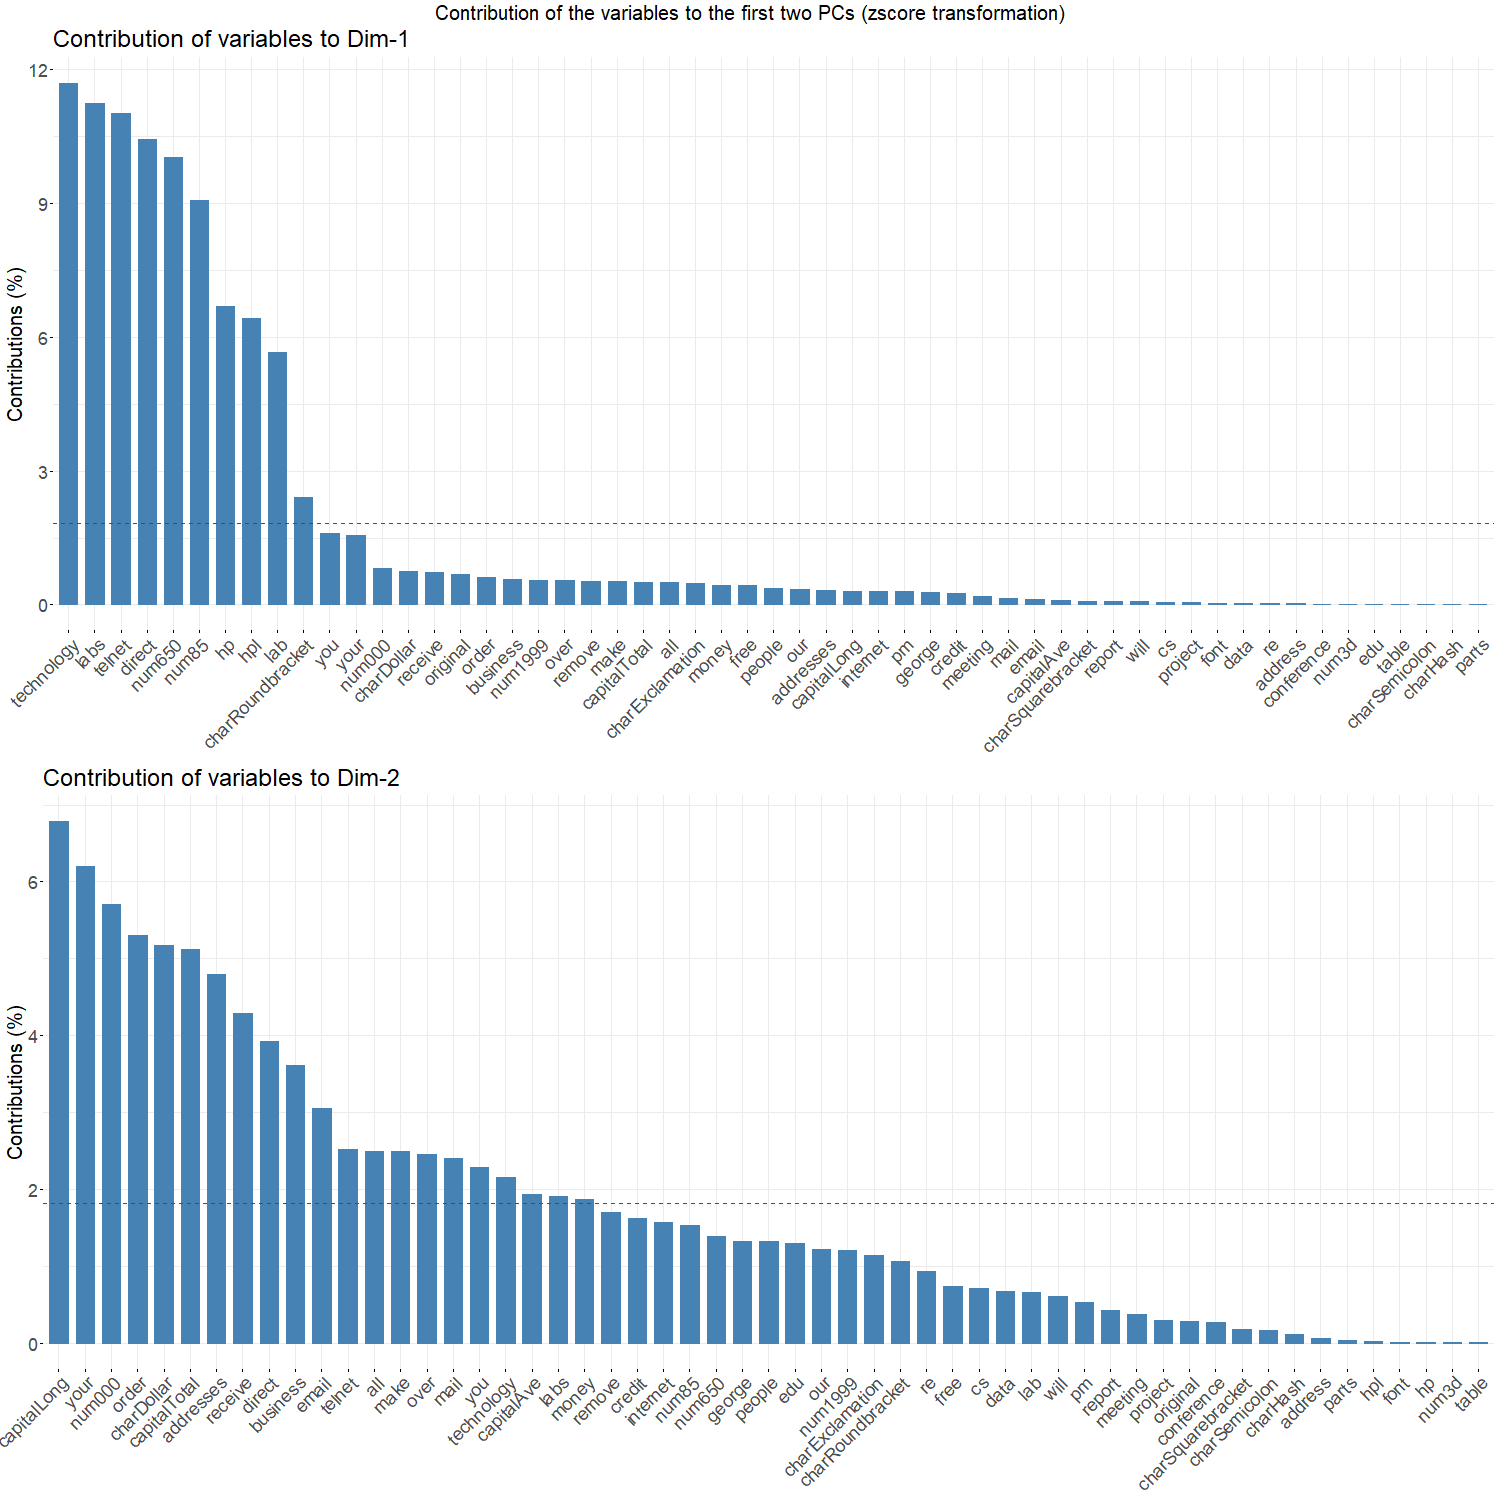
\includegraphics[width=0.9\textwidth]{proj2_plots/varplot2.png}
		\caption{PCA results for standardized data (variable contribution plot)}
		\label{fig::varplot_zscore}
	\end{figure}
	
	
	\begin{figure}[h]
		\centering
		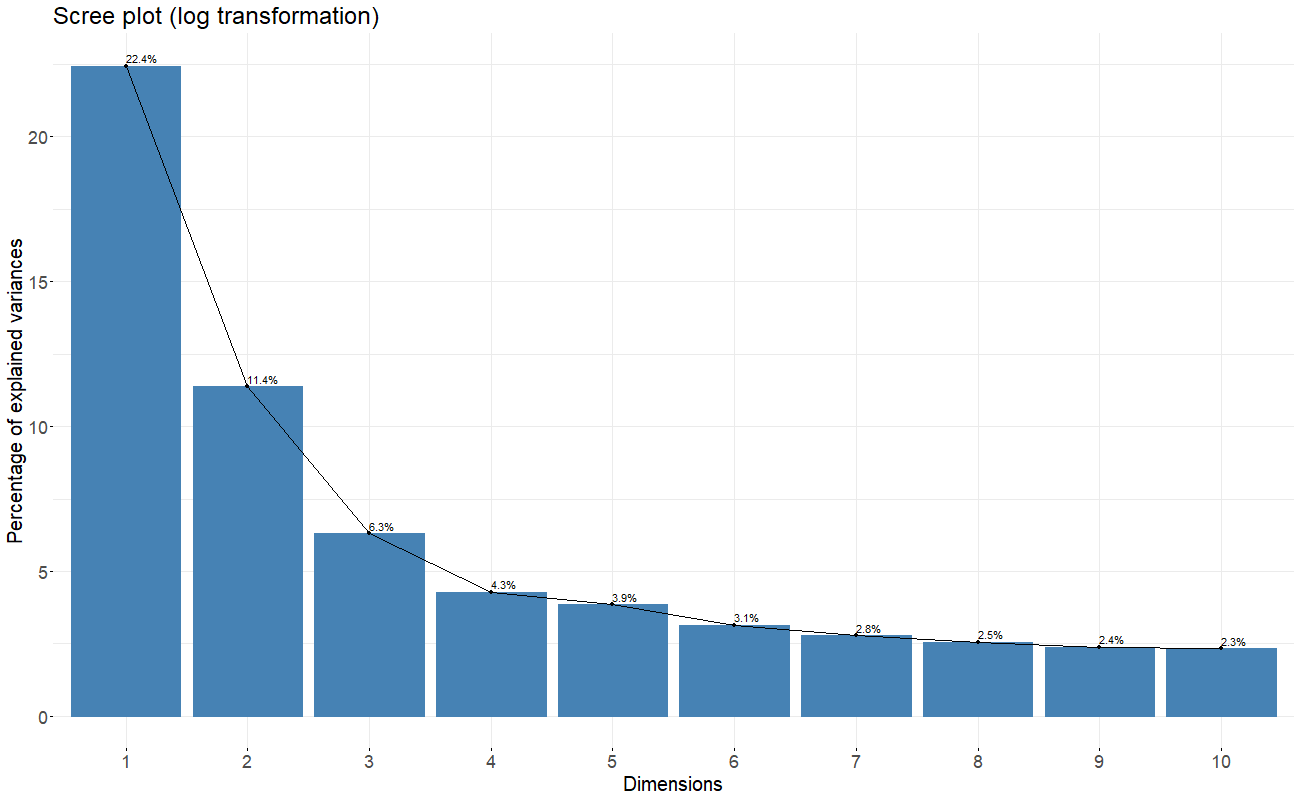
\includegraphics[width=0.9\textwidth]{proj2_plots/screeplot3.png}
		\caption{PCA results for log-transformed data (scree plot)}
		\label{fig::screeplot_log}
	\end{figure}
	
	\begin{figure}[h]
		\centering
		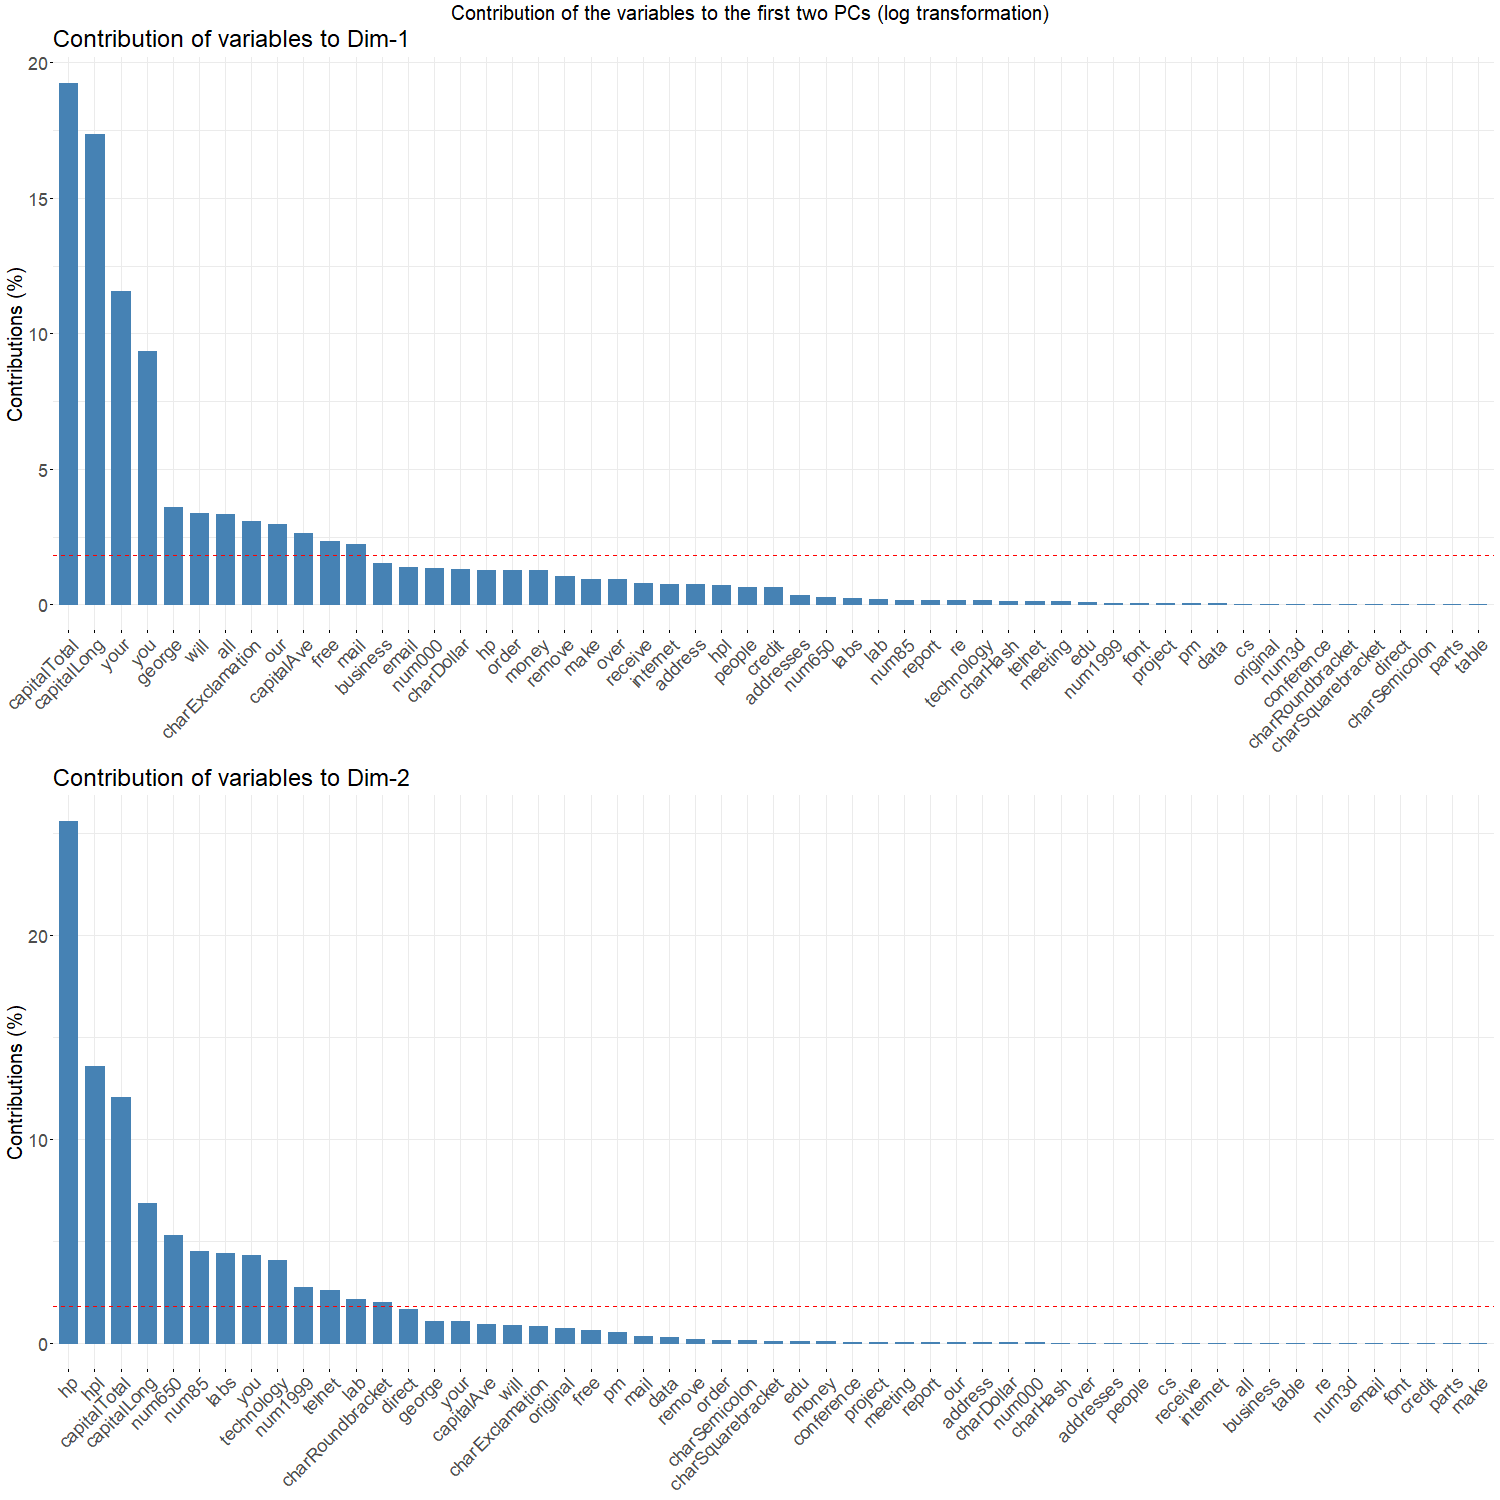
\includegraphics[width=0.9\textwidth]{proj2_plots/varplot3.png}
		\caption{PCA results for log-transformed data (variable contribution plot)}
		\label{fig::varplot_log}
	\end{figure}
	
	Results for log-transformed data can be seen on Figure \ref{fig::screeplot_log} (scree plot) and Figure \ref{fig::varplot_log} (variable contribution plot).
	Here again we observe that contribution of many variables is higher than for original data. Also we see that in comparison to z-score transformed data we will probably be able to eliminate more principal components for the latter analysis.
	
	To reduce dimensionality of our data using PCA, for both data transformations we selected a method based on feature variance. First, we compute
	mean standard deviation across all principal components. Second, we check which PCs display lower standard deviation than the computed mean. Finally,
	we reject those PCs falling below threshold -- as a result, we obtain 26 principal components for z-score standardized data and 19 of them for log-transformed data.
	This seems like a really good reduction in dimensionality, considering that we started off with as much as 55 features! 
	
	\section{Clustering}
	For cluster analysis we will use k-means, PAM and AGNES algorithms for transformed \textit{Spambase} datasets and also for datasets built using principal components extracted while performing PCA. 
	First thing we need to do before applying the algorithms is checking the optimal number of clusters $k$ for each of them.
	In case of k-means and PAM, we will do it by calculating the silhouette index, and for AGNES we will select the number of clusters by analysing the dendrogram.
	Given the fact that the main goal of our analysis is to check how well the clustering algorithms will be able to differentiate between spam and non-spam e-mails,
	we expect the optimal number of clusters to be $k=2$, but of course we cannot eliminate other possibilities, as there might be some hidden data structures within our 
	dataset which should not be omitted.
	
	Let us first take a look at silhouette index values for k-means without PCA, shown on Figure \ref{fig::clust_num_kmeans}. We see that for the z-score standardized
	data we should extract 2 clusters, while for the log-transformed data the optimal number of clusters is 3. The same is observed for k-means with PCA (Figure \ref{fig::clust_num_keans_pca}).
	Situation changes slightly in case of PAM algorithm -- here, the silhouette index method picked $k=2$ for both data transformations without PCA (Figure \ref{fig::clust_num_pam}),
	and for PCA $k=3$ (Figure \ref{fig::clust_num_pam_pca}).

	When it comes to AGNES, the choice of the optimal number of clusters is less obvious. Looking at the dendrogram, we need to pick such $k$ that the increase
	in between-cluster dissimilarity from $k$ clusters to $k+1$ clusters is significantly less than the increase in between-cluster dissimilarity from $k-1$ clusters to $k$ clusters.
	From Figure \ref{fig::clust_num_agnes_scaled} we see that for z-score standardized data without PCA $k=2$ would be a good choice ($k=3$ to include outliers as separate cluster),
	and the same with PCA (Figure \ref{fig::clust_num_agnes_scaled_pca}). For log-transformed data, both without PCA (Figure \ref{fig::clust_num_agnes_log}) and with PCA
	(Figure \ref{fig::clust_num_agnes_log_pca}), the optimal number of clusters is evaluating to 3. As expected, in case of the second data transformation we don't observe any outliers dectected by AGNES.

	
	\begin{figure}[h]
		\centering
		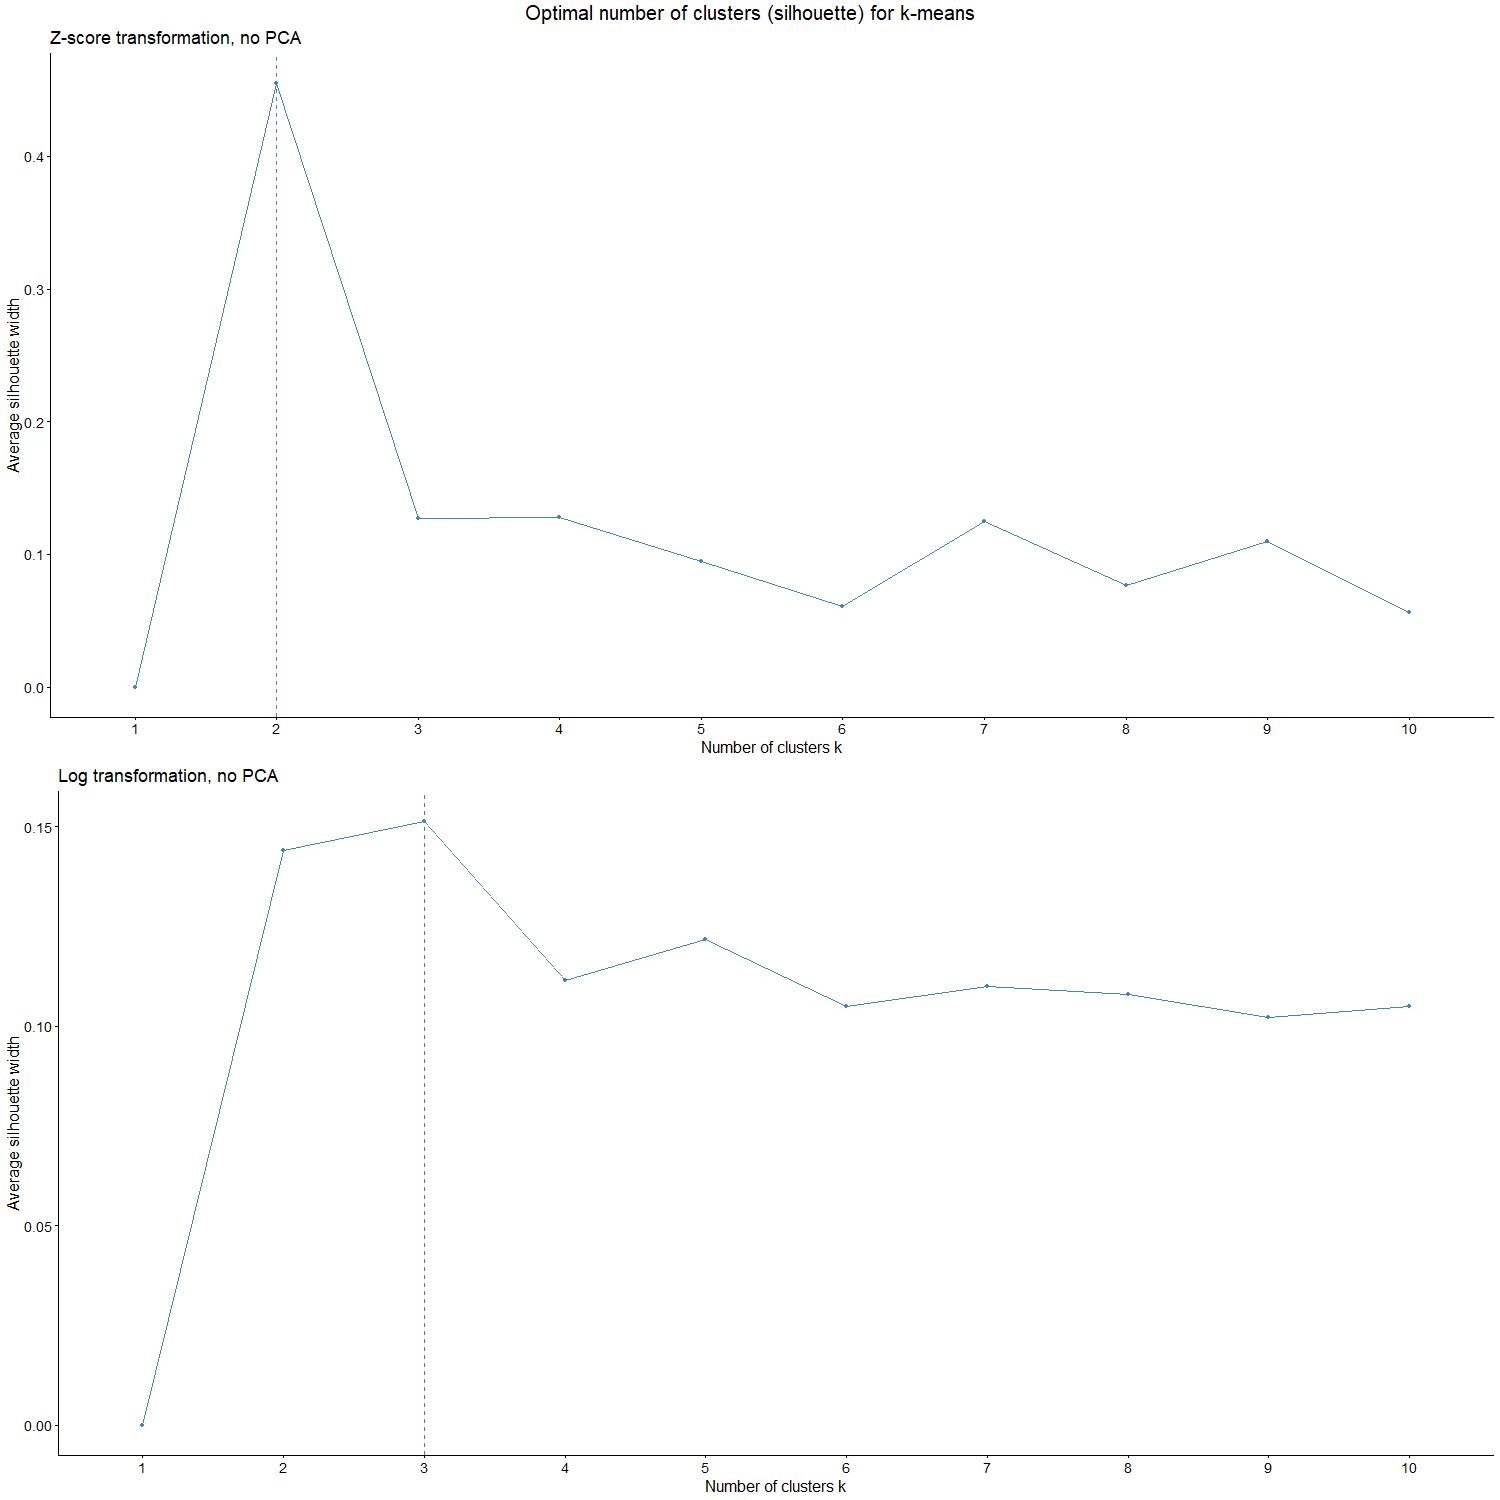
\includegraphics[width=0.9\textwidth]{proj2_plots/kmeans_clust_num.png}
		\caption{Number of clusters for k-means (no PCA)}
		\label{fig::clust_num_kmeans}
	\end{figure}

	\begin{figure}[h]
		\centering
		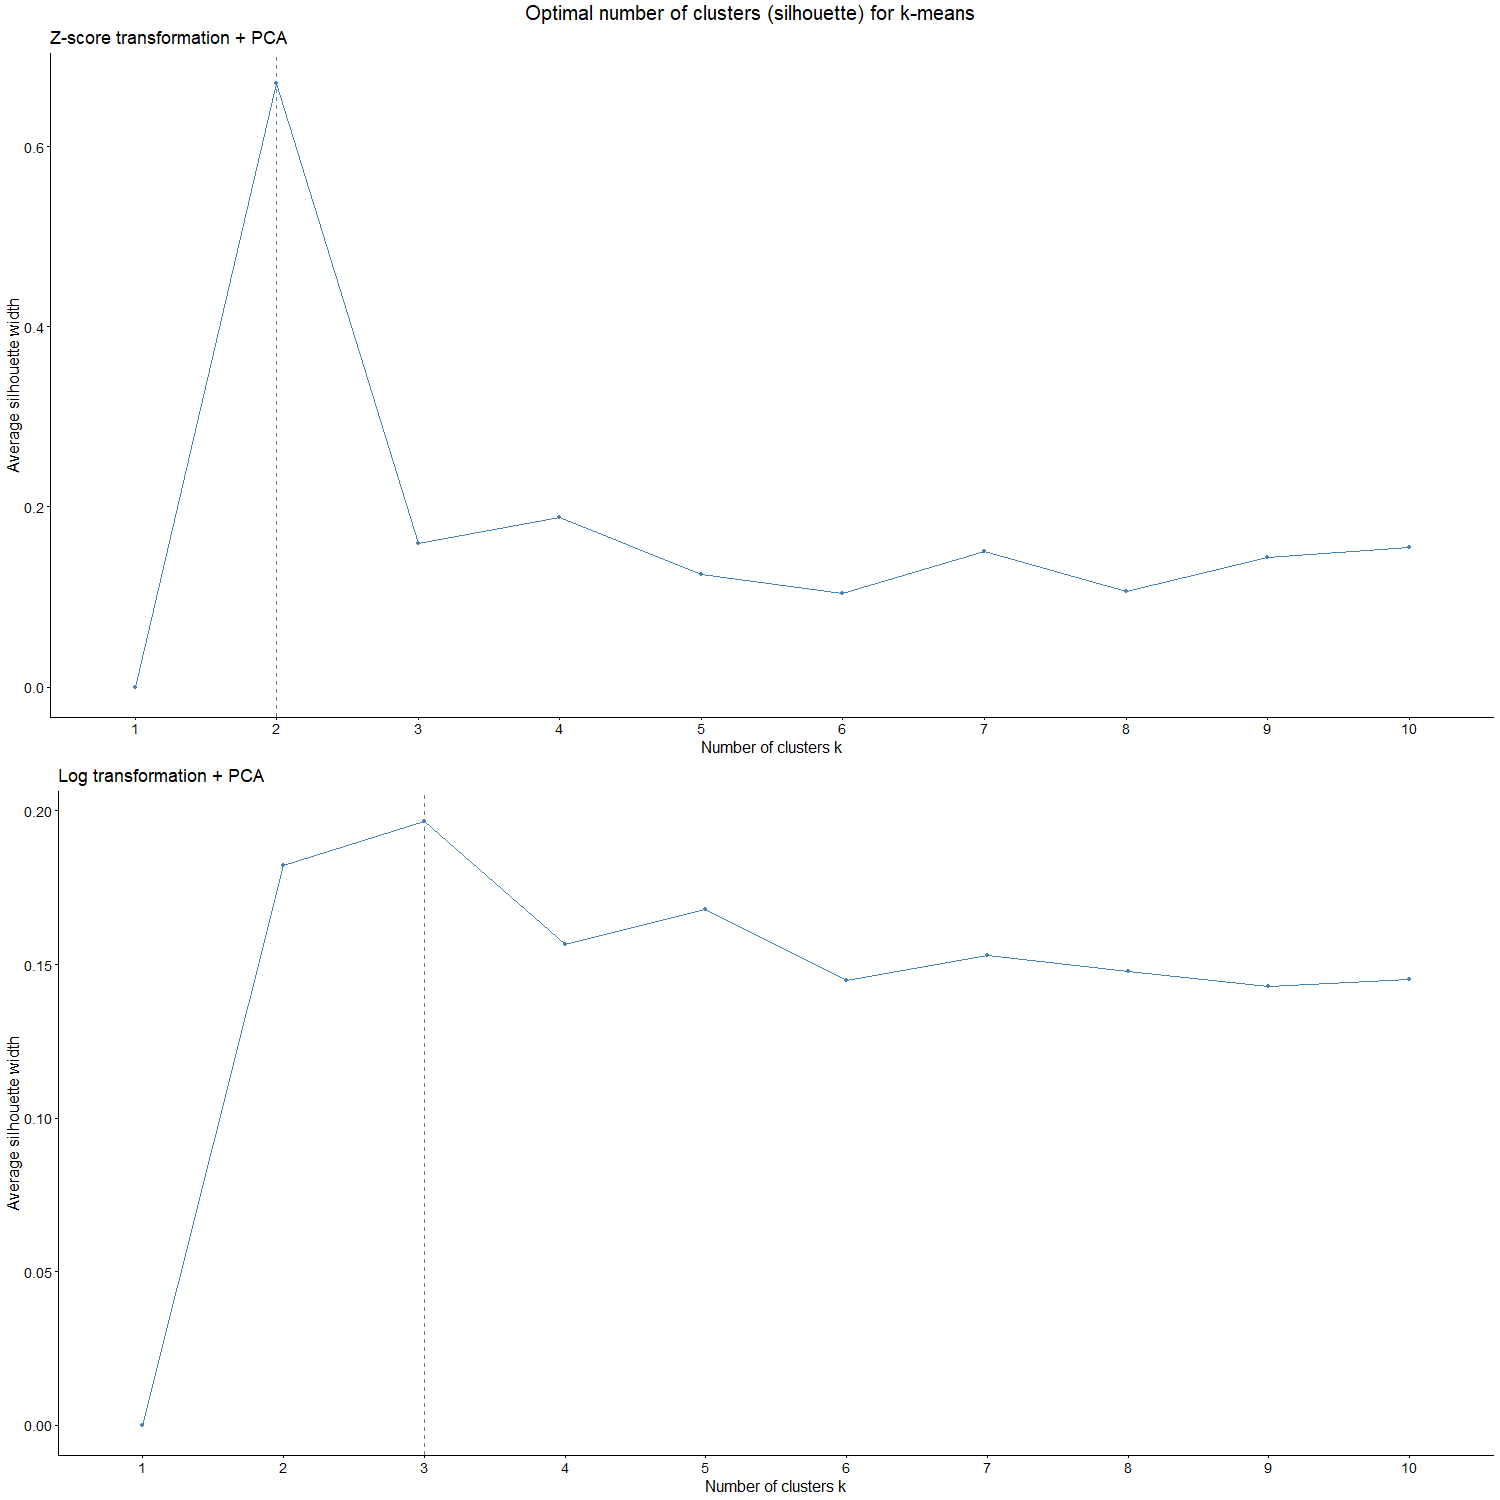
\includegraphics[width=0.9\textwidth]{proj2_plots/kmeans_clust_num_pca.png}
		\caption{Number of clusters for k-means (with PCA)}
		\label{fig::clust_num_keans_pca}
	\end{figure}
	
	\begin{figure}[h]
		\centering
		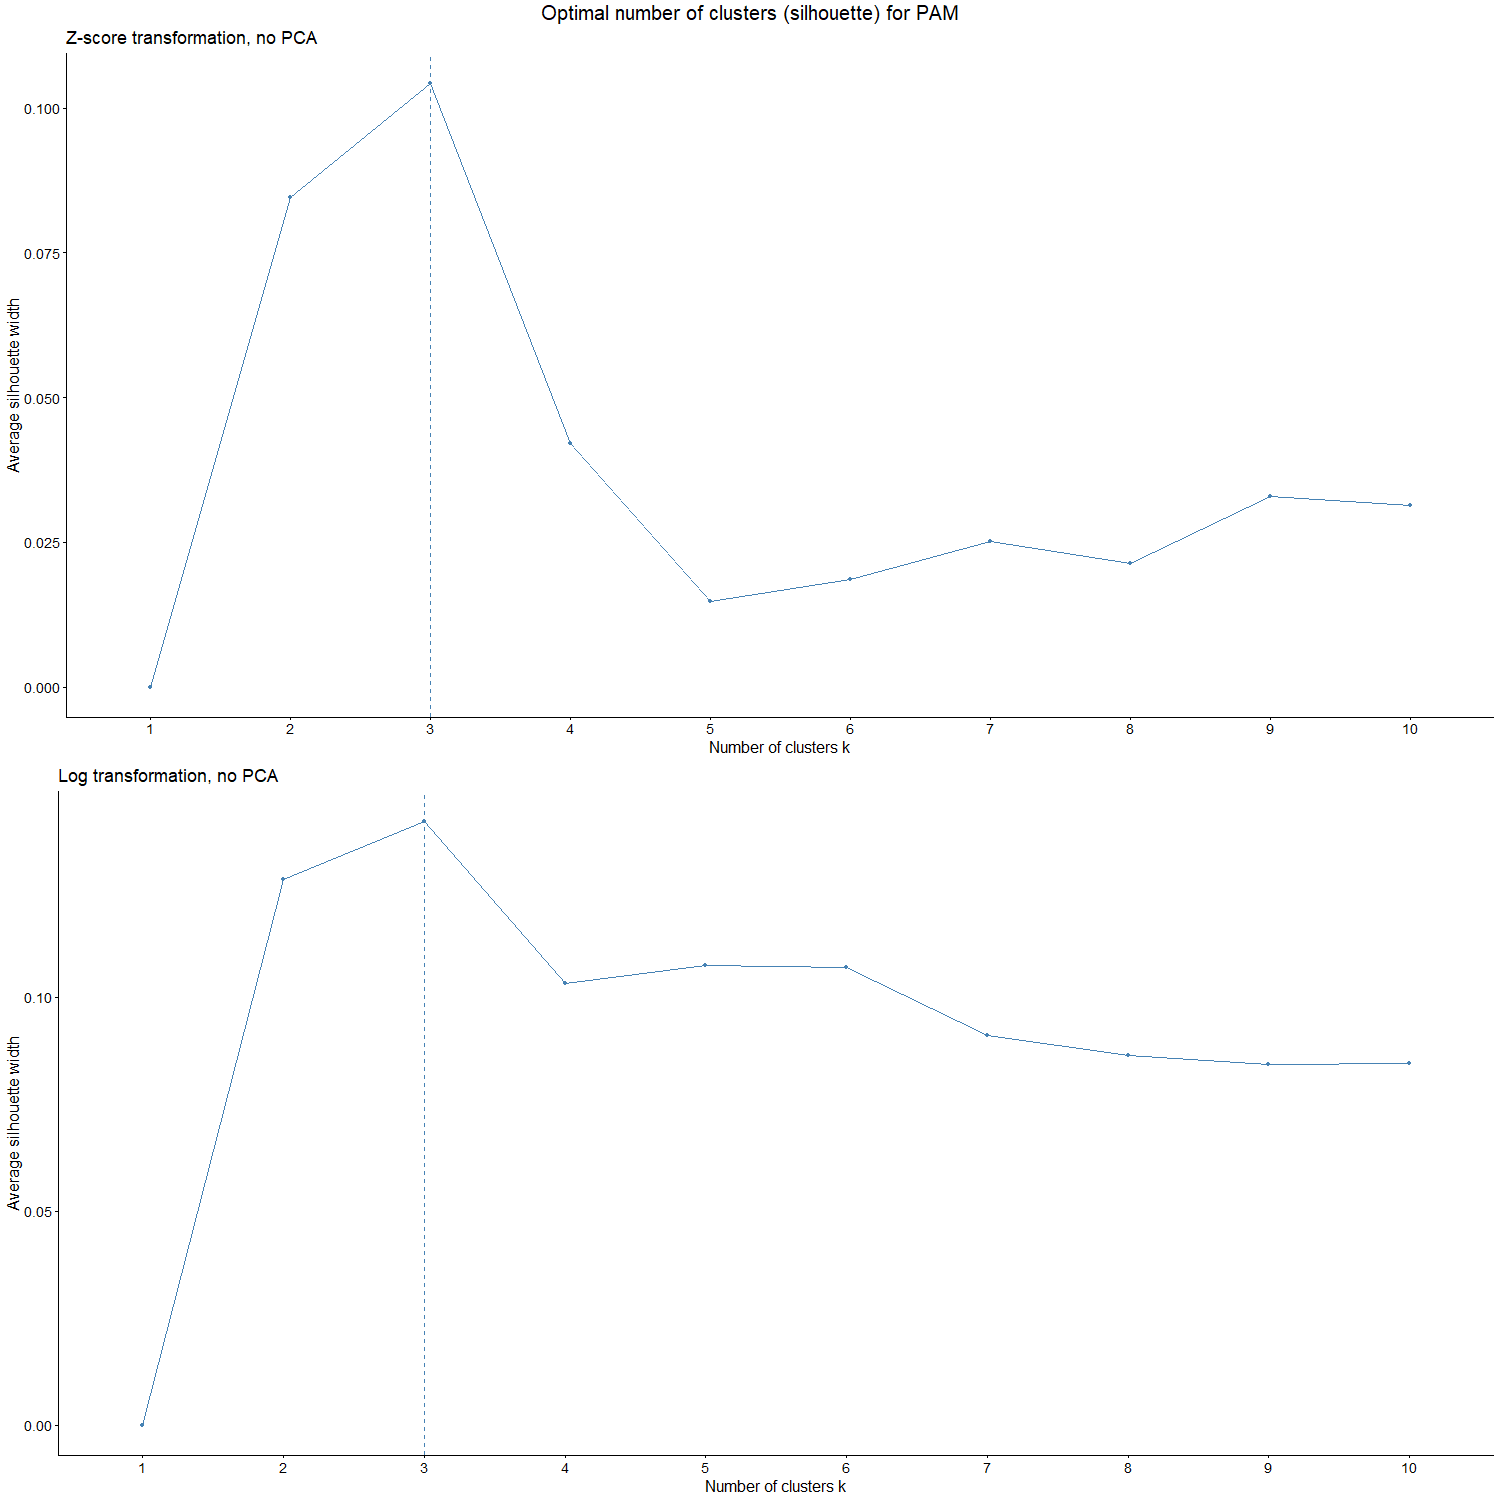
\includegraphics[width=0.9\textwidth]{proj2_plots/pam_clust_num.png}
		\caption{Number of clusters for PAM (no PCA)}
		\label{fig::clust_num_pam}
	\end{figure}
	
	\begin{figure}[h]
		\centering
		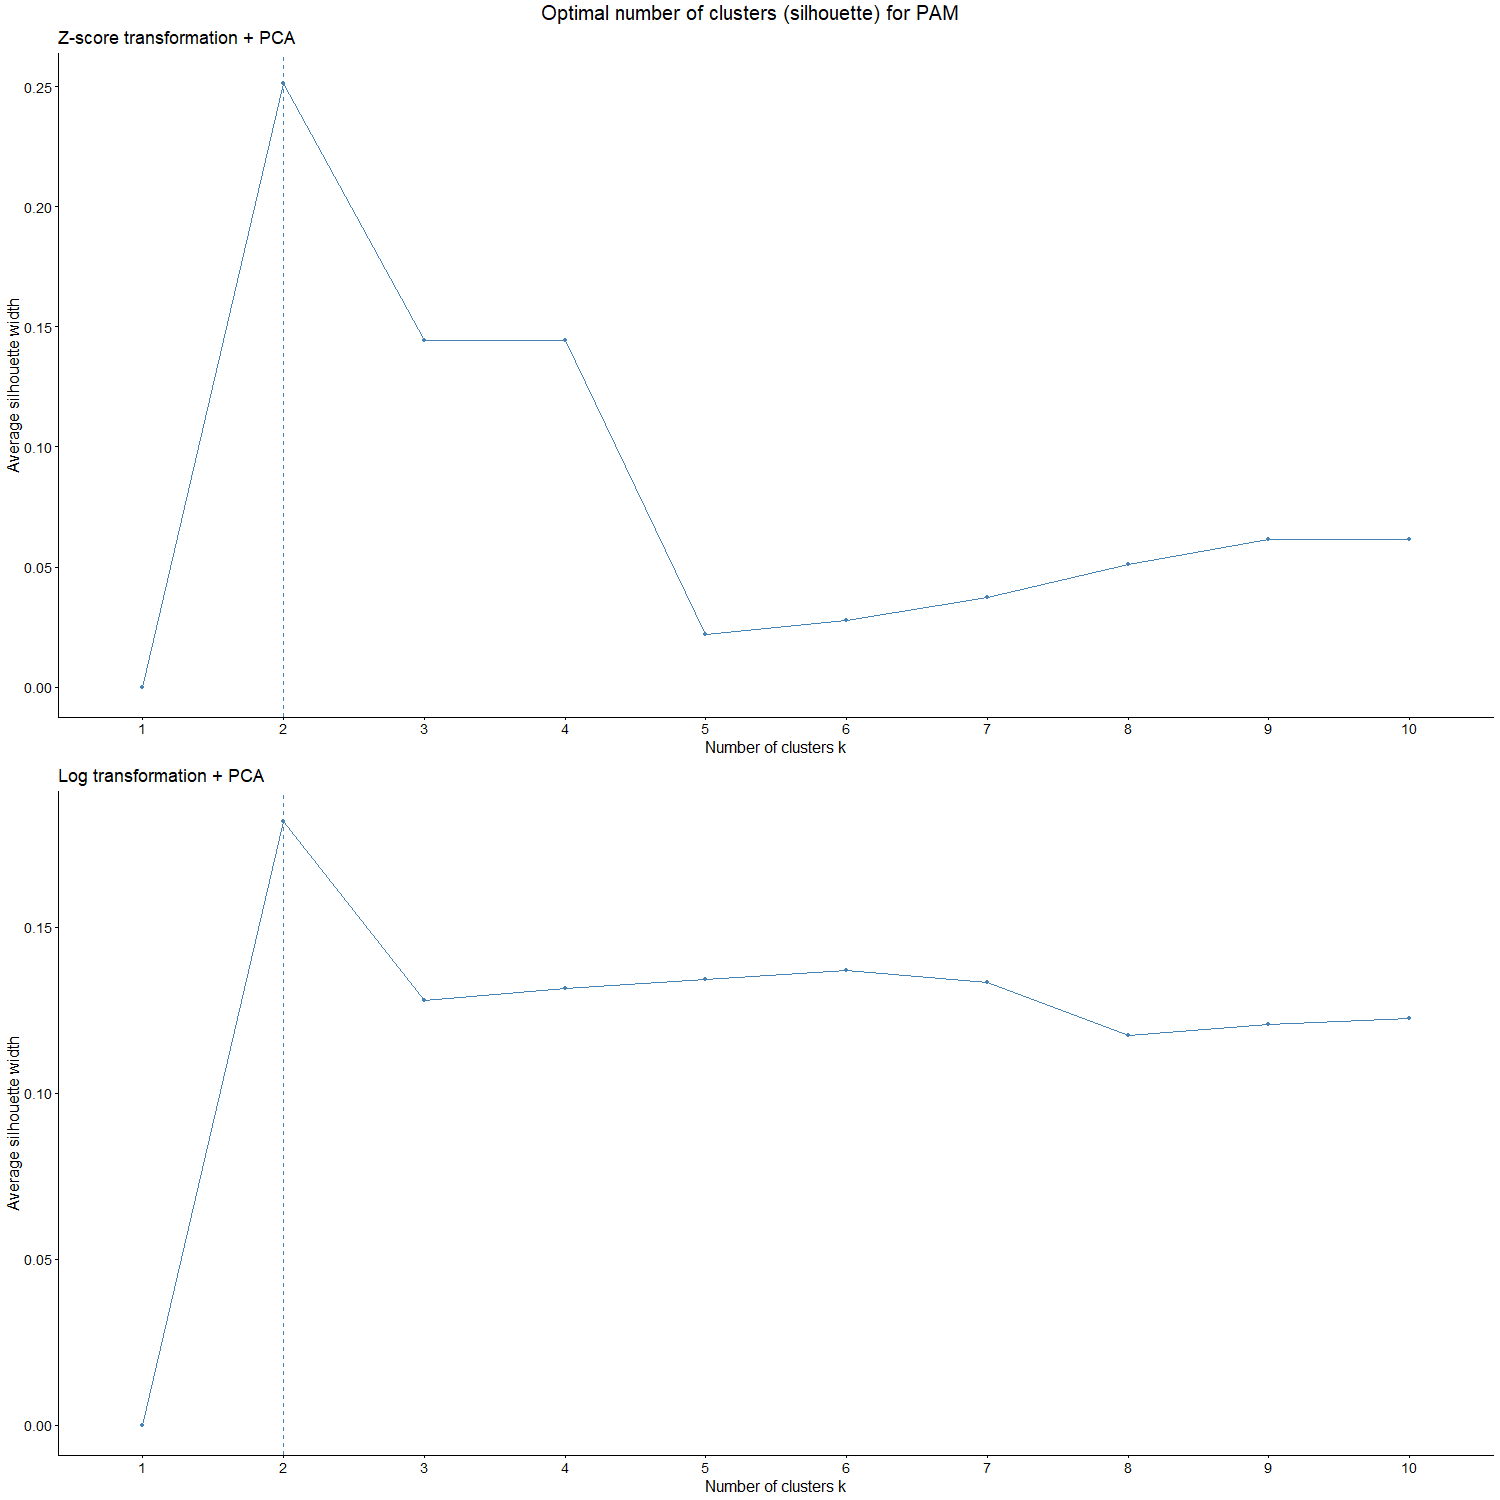
\includegraphics[width=0.9\textwidth]{proj2_plots/pam_clust_num_pca.png}
		\caption{Number of clusters for PAM (with PCA)}
		\label{fig::clust_num_pam_pca}
	\end{figure}

	\begin{figure}[h]
		\centering
		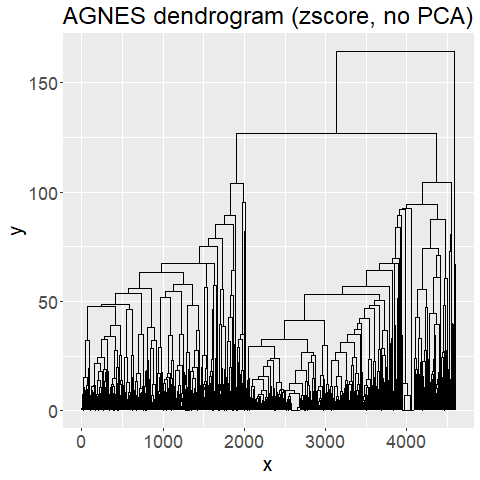
\includegraphics[width=0.9\textwidth]{proj2_plots/dendro_scaled_nopca.png}
		\caption{Number of clusters for AGNES (no PCA)}
		\label{fig::clust_num_agnes_scaled}
	\end{figure}

	\begin{figure}[h]
		\centering
		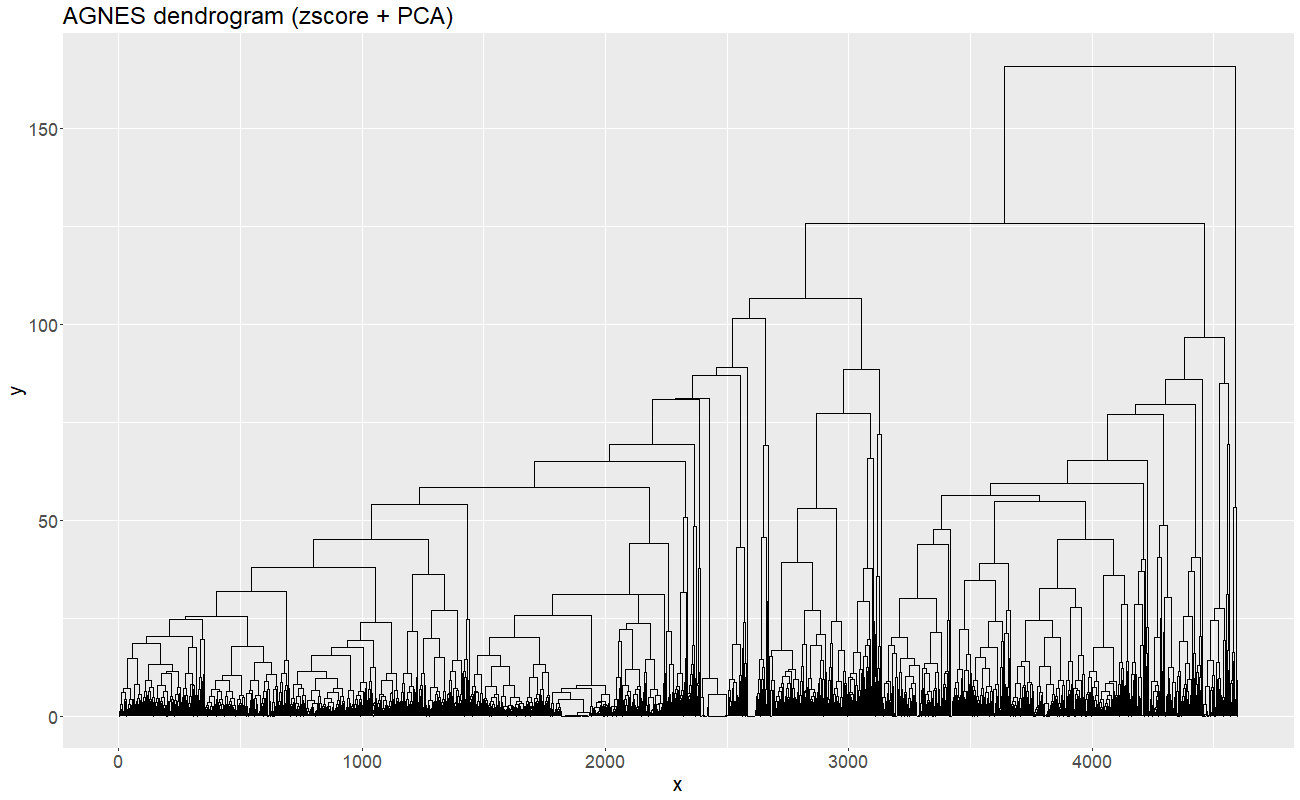
\includegraphics[width=0.9\textwidth]{proj2_plots/dendro_scaled_pca.png}
		\caption{Number of clusters for AGNES (with PCA)}
		\label{fig::clust_num_agnes_scaled_pca}
	\end{figure}

	\begin{figure}[h]
		\centering
		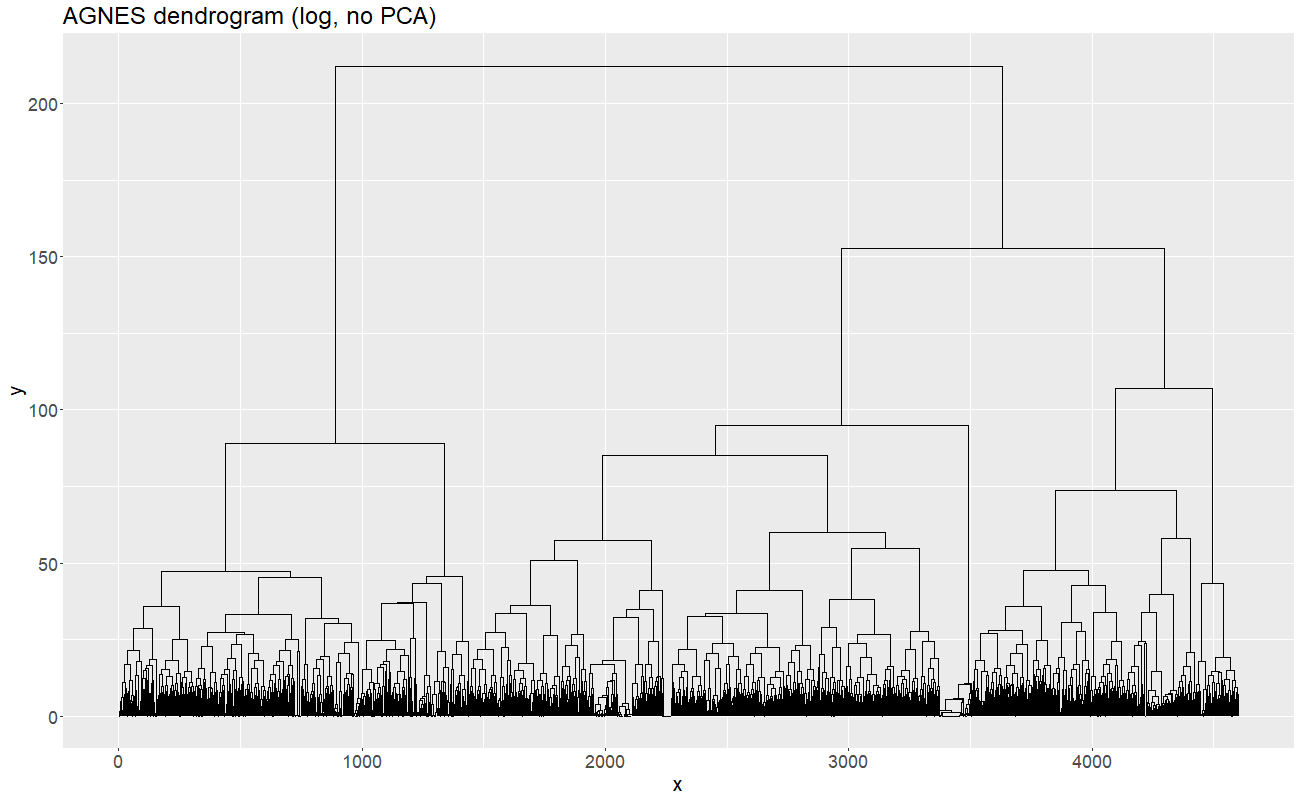
\includegraphics[width=0.9\textwidth]{proj2_plots/dendro_log_nopca.png}
		\caption{Number of clusters for AGNES (no PCA)}
		\label{fig::clust_num_agnes_log}
	\end{figure}

	\begin{figure}[h]
		\centering
		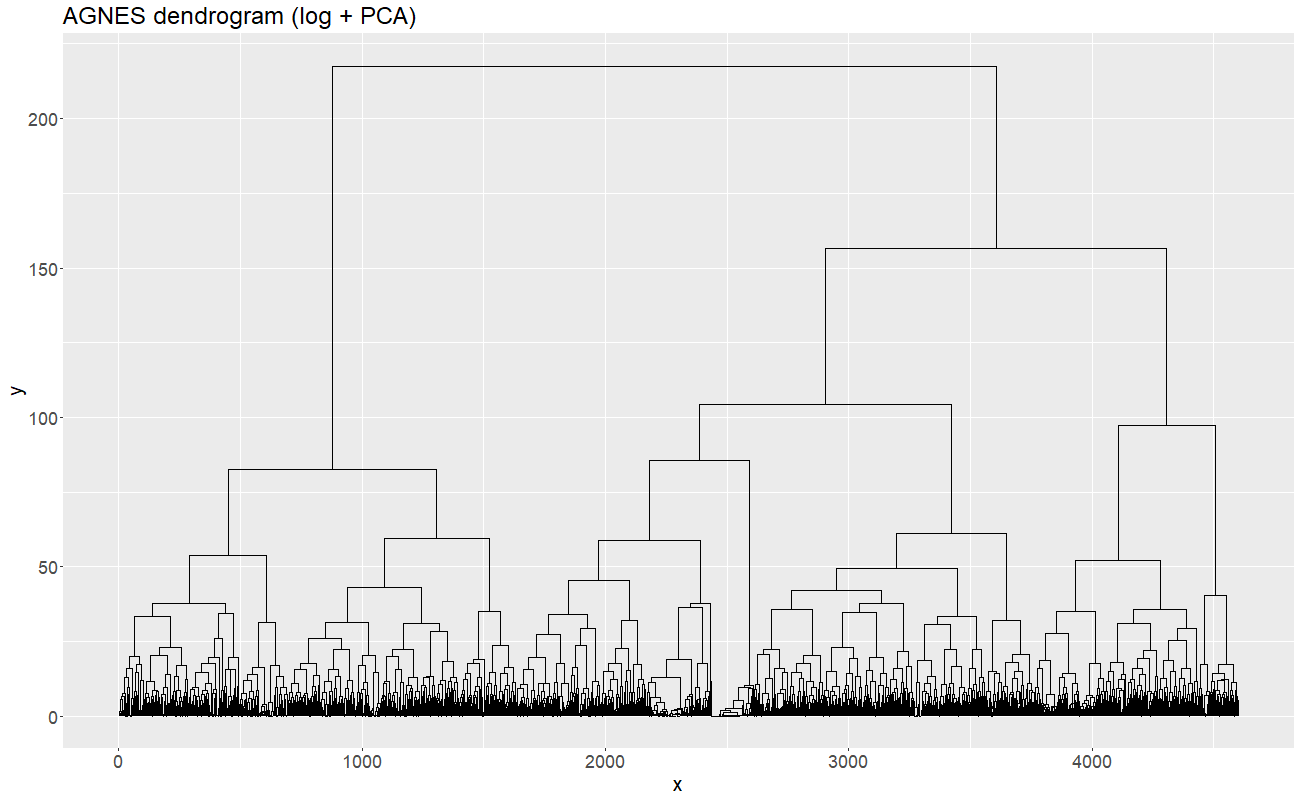
\includegraphics[width=0.9\textwidth]{proj2_plots/dendro_log_pca.png}
		\caption{Number of clusters for AGNES (with PCA)}
		\label{fig::clust_num_agnes_log_pca}
	\end{figure}
	
	Once we have selected the optimal number of clusters $k$ for all algorithms, we can 
	move on to clustering. In the following subsections, we will discuss the results obtained for 
	k-means, PAM and AGNES.
	
	\subsection{k-means}

	Figure \ref{fig::clust_kmeans_scaled} shows the results of clustering with k-means for z-score transformed data without PCA.
	We can see from this plot that cluster number 1 contains much more observations than the cluster number 2.
	Moreover, it looks like the nonspam class dominates in both of the clusters. We can verify this by looking at Table \ref{tab::clust_kmeans_scaled} --
	most observations from both classes fall into the first cluster, so this time the k-means algorithm wasn't able to differentiate well between spam and nonspam messages.
	What's interesting, applying PCA did not change the results much for the standardized data. Both Figure \ref{fig::clust_kmeans_scaled_pca}
	and Table \ref{tab::clust_kmeans_scaled_pca} display results almost identical to those observed in the previous case. 

	\begin{figure}[h]
		\centering
		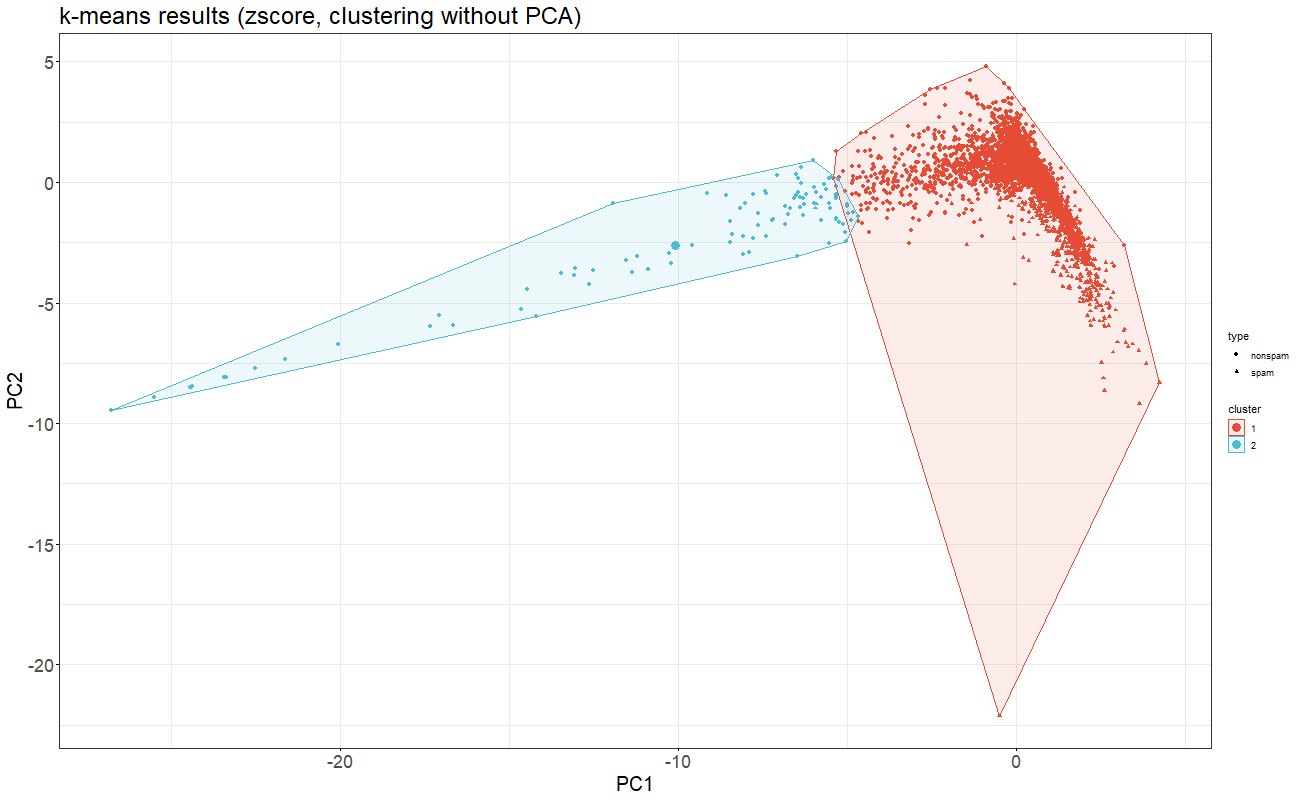
\includegraphics[width=0.9\textwidth]{proj2_plots/kmeans_res_scaled.png}
		\caption{Clustering with k-means (z-score, no PCA)}
		\label{fig::clust_kmeans_scaled}
	\end{figure}

	\begin{table}[h]
		\centering
		\begin{tabular}{lcc}
			& \multicolumn{2}{c}{\textbf{Type}} \\
			\textbf{Cluster} & \textbf{nonspam} & \textbf{spam} \\
			\textbf{1} & 2676 & 1811 \\
			\textbf{2} & 112 & 2 \\
		\end{tabular}
		\caption{Clustering with k-means (z-score, no PCA)}
		\label{tab::clust_kmeans_scaled}
	\end{table}

	\begin{figure}[h]
		\centering
		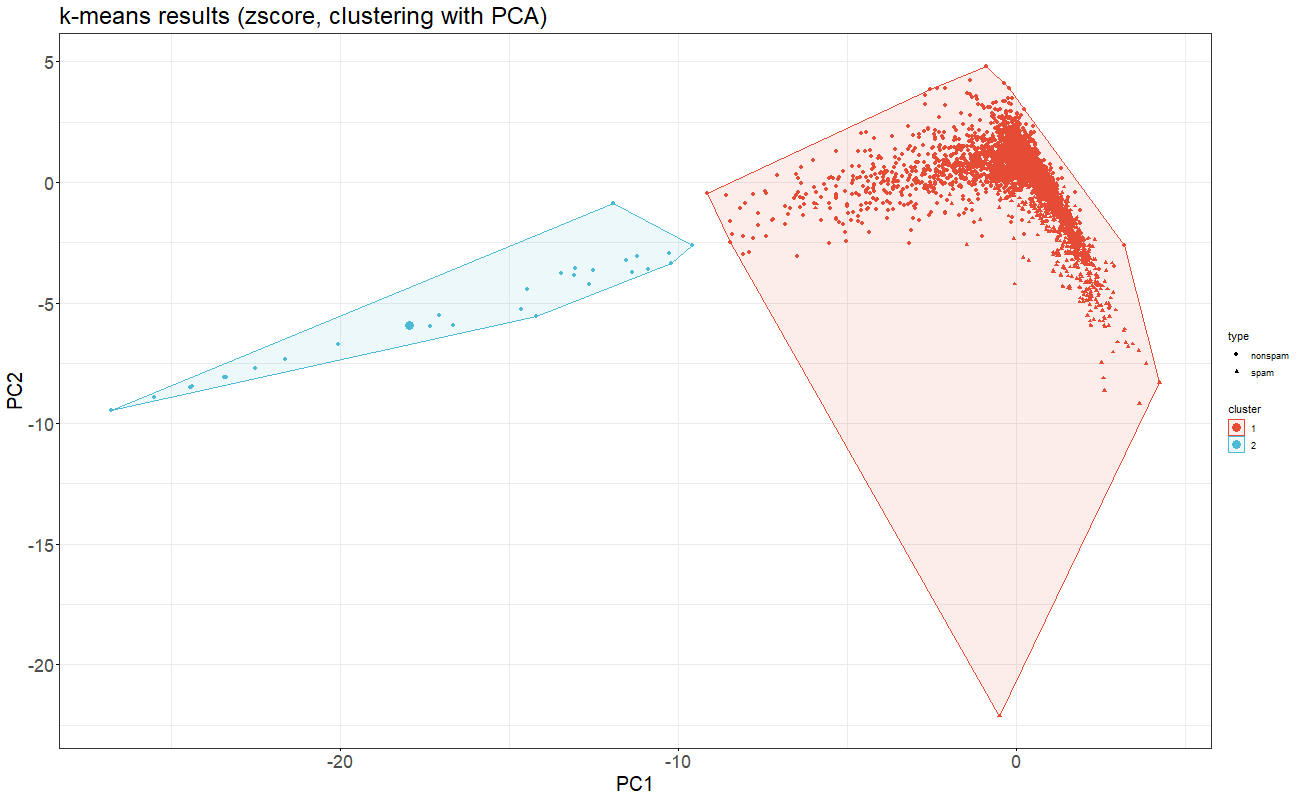
\includegraphics[width=0.9\textwidth]{proj2_plots/kmeans_res_scaled_pca.png}
		\caption{Clustering with k-means (z-score with PCA)}
		\label{fig::clust_kmeans_scaled_pca}
	\end{figure}

	\begin{table}[h]
		\centering
		\begin{tabular}{lcc}
			& \multicolumn{2}{c}{\textbf{Type}} \\
			\textbf{Cluster} & \textbf{nonspam} & \textbf{spam} \\
			\textbf{1} & 2751 & 1813 \\
			\textbf{2} & 37 & 0 \\
		\end{tabular}
		\caption{Clustering with k-means (z-score with PCA)}
		\label{tab::clust_kmeans_scaled_pca}
	\end{table}

	Situation looks quite different for the log-transformed data. Figure \ref{fig::clust_kmeans_log} shows cluster assignment for the
	no-PCA case. We see that the cluster number 3 contains mostly nonspam class, while the other two clusters consist mainly of spam, and
	Table \ref{tab::clust_kmeans_log} confirms that. Very similar situation is observed for log-transformed data with PCA. From Figure
	\ref{fig::clust_kmeans_log_pca} we see that the cluster assignment didn't change much, except the names for cluster 1 and cluster 2 are swapped.
	Also looking at Table \ref{tab::clust_kmeans_log_pca} we can say that the proportions of classes assigned to particular clusters is almost identical
	as in the previous case, so again we don't observe much influence on clustering from applying PCA to our data, but we can certainly say
	that it is much easier for k-means to differentiate between spam and nonspam in case of log-transformation rather than for the z-score scaling.

	\begin{figure}[h]
		\centering
		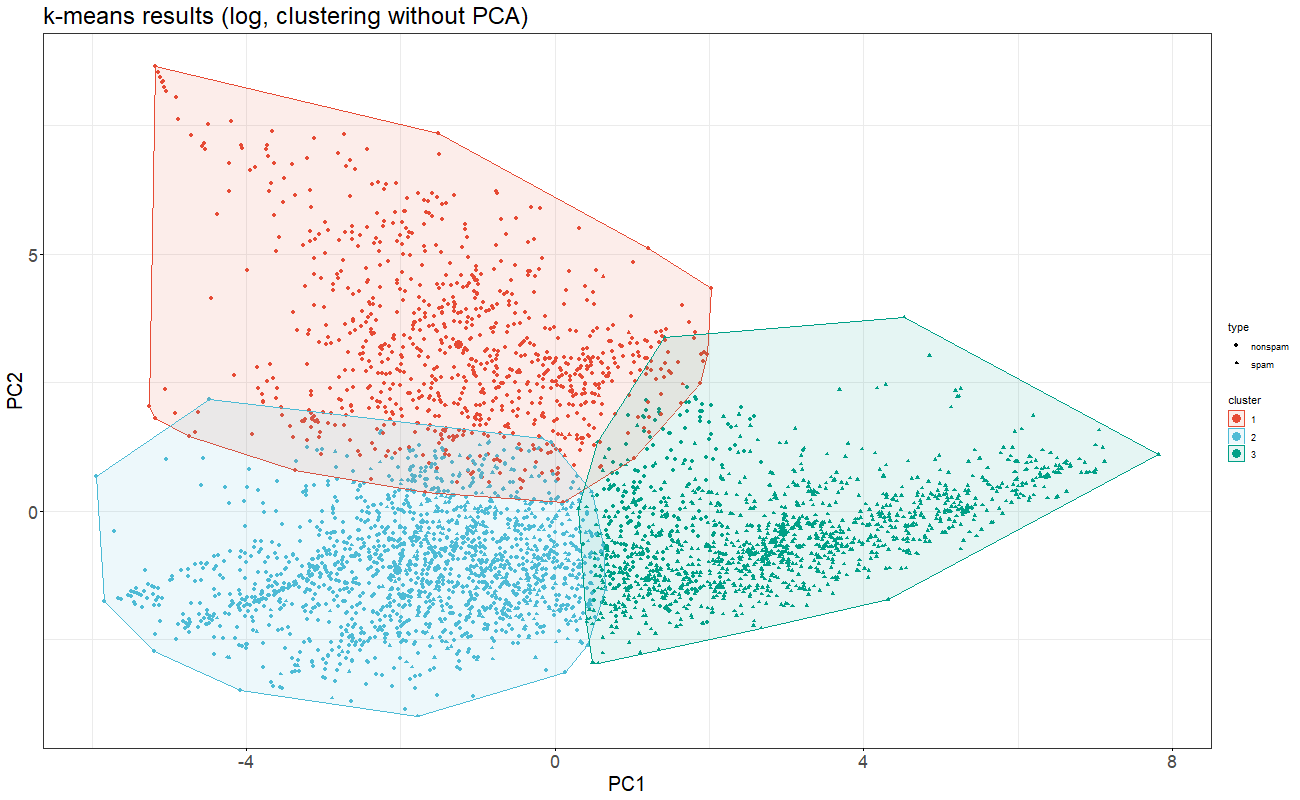
\includegraphics[width=0.9\textwidth]{proj2_plots/kmeans_res_log.png}
		\caption{Clustering with k-means (log, no PCA)}
		\label{fig::clust_kmeans_log}
	\end{figure}

	\begin{table}[h]
		\centering
		\begin{tabular}{lcc}
			& \multicolumn{2}{c}{\textbf{Type}} \\
			\textbf{Cluster} & \textbf{nonspam} & \textbf{spam} \\
			\textbf{1} & 900 & 11 \\
			\textbf{2} & 1626 & 326 \\
			\textbf{3} & 262 & 1476 \\
		\end{tabular}
		\caption{Clustering with k-means (log, no PCA)}
		\label{tab::clust_kmeans_log}
	\end{table}

	\begin{figure}[h]
		\centering
		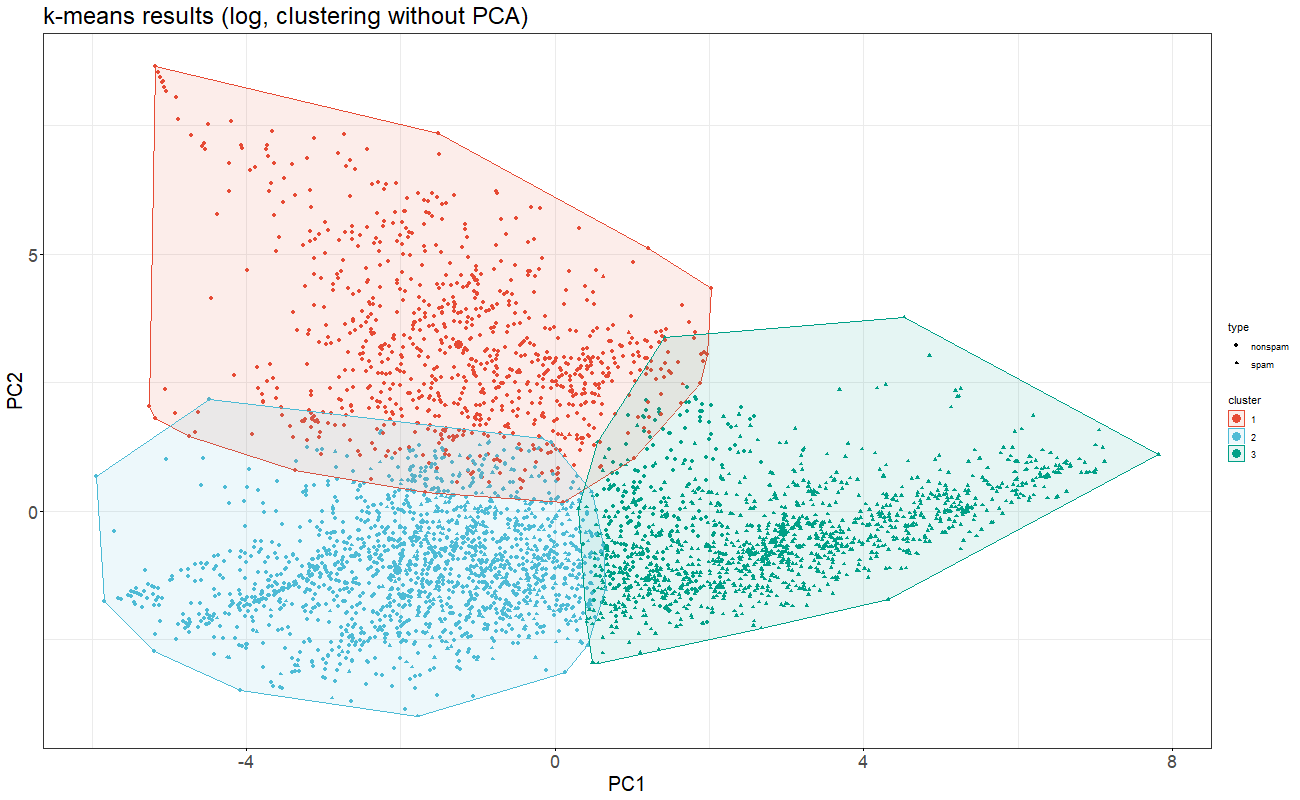
\includegraphics[width=0.9\textwidth]{proj2_plots/kmeans_res_log.png}
		\caption{Clustering with k-means (log with PCA)}
		\label{fig::clust_kmeans_log_pca}
	\end{figure}

	\begin{table}[h]
		\centering
		\begin{tabular}{lcc}
			& \multicolumn{2}{c}{\textbf{Type}} \\
			\textbf{Cluster} & \textbf{nonspam} & \textbf{spam} \\
			\textbf{1} & 1628 & 328 \\
			\textbf{2} & 893 & 11 \\
			\textbf{3} & 267 & 1474 \\
		\end{tabular}
		\caption{Clustering with k-means (log with PCA)}
		\label{tab::clust_kmeans_log_pca}
	\end{table}
	
	\subsection{PAM}
	
	\subsection{AGNES}
	 
\end{document}